\chapter{INTRODUCCIÓN}
\label{ch:intro}
En el presente capítulo se hace una descripción detallada del contexto del proyecto de título. Junto a esto, se presenta la oportunidad y los objetivos e ideas generales que se abordarán.

\section{Contexto}
La educación ha sido un tema muy importante a lo largo de la historia y más aún en la actualidad, ya que además de ser un derecho humano fundamental, es una herramienta mediante la cual es posible otorgarle a la sociedad considerables beneficios, con el fin de generar una sociedad mejor, lo que permite que el país se desarrolle gracias a la sociedad de calidad que la conforma. \\

%La educación ha sido un tema muy importante a lo largo de la historia y más aún en la actualidad, ya que además de ser un derecho humano fundamental, es una herramienta mediante la cual es posible otorgarle a la sociedad considerables beneficios, no solamente la oportunidad de acceder a buenos puestos de trabajos con abundantes salarios, sino que también permite que el país se desarrolle gracias a la sociedad de calidad que la conforma. 

Los estudios demuestran que \cite{unicef}:
\begin{itemize}
\item Proveer a todos los niños y niñas de una educación básica de calidad podría impulsar el crecimiento económico anual en un 2\% en los países de bajos ingresos.
\item Sería posible librar de la pobreza al 12\% de las personas pobres (más de 170 millones) si todos los estudiantes de los países pobres tuvieran aptitudes de lectura básicas.
\item Que durante las últimas cuatro décadas, el incremento mundial que ha experimentado la educación de las mujeres ha evitado más de cuatro millones de muertes infantiles.
\item Que cada año adicional de escolarización puede propiciar un aumento de los ingresos de la mujer de entre el 10\% y el 20\%.
\item Que 1 millón de dólares invertidos en educación y aptitudes equivale a 10 millones de crecimiento económico.
\end{itemize}

Es por esto que la educación resulta ser importante para el desarrollo de un país, y para que esto se cumpla un punto muy importante es fomentar la retención escolar, es decir, evitar las fugas del sistema educativo. 

\subsection{El Sistema de Educación en Chile}
Para comenzar, se procederá a describir el sistema de educación en Chile, su estructura y organización.

El Sistema Escolar Chileno está compuesto por niveles de enseñanza, que son diferentes etapas del proceso educativo y buscan asegurar y facilitar la continuidad a lo largo del tiempo. \\

Los niveles de enseñanza son los siguientes:

\begin{enumerate}
    \item Educación Parvularia: es el primer nivel educativo, recibe a niños y niñas de hasta 5 años de edad en salas cunas, Nivel Medio Menor, Nivel Medio Mayor y Primer y Segundo  Nivel de Transición. 
    La finalidad de la educación parvularia es principalmente promover el desarrollo de la personalidad de los niños, facilitar el proceso de sociabilización y prepararlos para enfrentar con éxito los siguientes niveles educativos.
    \item Educación Básica: este nivel corresponde al primer periodo escolar, comprende 8 años de educación obligatoria y recibe a niños de entre 6 y 13 años. A su vez, se divide en dos ciclos: primer ciclo básico, desde 1ero a 4to básico; y segundo ciclo básico, desde 5to a 8vo básico.
    El objetivo es incentivar el desarrollo integral de la personalidad del alumno, estimular su creatividad para su integración gradual como sujeto activo en la sociedad.
    \item Educación Media: es el último periodo escolar, tiene una duración de 4 años y recibe a quienes egresan de la educación básica. Quienes cursan este período tienen entre 14 y 18 años. Cabe mencionar que este nivel puede tener dos modalidades: educación media científico-humanista, que tiene como objetivo formar integralmente a los estudiantes para que continúen estudios superiores o se integren al campo laboral; y la educación técnico profesional, orientada a formar integralmente a los estudiantes y prepararlos como técnicos a nivel medio para desempeñarse en las áreas de producción o servicios del sector laboral.
    \item Educación Superior: recibe a quienes egresan de la educación media. Está conformado oficialmente por Universidades, Institutos Profesionales, Centros de Formación Técnica y Establecimientos de Educación Superior de las Fuerzas Armadas, de Orden y Seguridad. 
\end{enumerate}

Con respecto a la gestión del Sistema Escolar Chileno, la administración de los establecimientos educacionales que imparten educación básica y media, es realizada por sostenedores, que son personas o instituciones municipales y particulares denominados ante el Estado, que tienen la responsabilidad del funcionamiento y la administración de las escuela y liceos. Dichos sostenedores son una figura jurídica que pueden administrar uno o varios establecimientos. 

De acuerdo a lo recién mencionado, existen tres tipos de instituciones que imparten la educación básica y media en el país:

\begin{itemize}
\item Instituciones Educacionales Municipales
\item Instituciones Educacionales Particulares Subvencionadas
\item Instituciones Educacionales Particulares Pagadas
\end{itemize}

La diferencia de cada administración radica principalmente en que los dos primeros reciben recursos por parte del Estado, las instituciones municipales en su totalidad y las particulares subvencionadas en un porcentaje. Por otro lado, los particulares son financiados en su totalidad por quienes asisten a el. 


\subsection{Institucionalidad del Sistema Educacional Chileno}
En esta sección se procederá a describir la institucionalidad del sistema educacional chileno. Esta estructura está formada por cuatro instituciones: el Ministerio de Educación, el Consejo Nacional de Educación, la Agencia de Calidad de la Educación y la Superintendencia de Educación. Sus funciones y relaciones se muestran de forma resumida en la Figura~\ref{fig:esquema}, que se muestra a continuación. 

\begin{figure}[H]
  \centering
    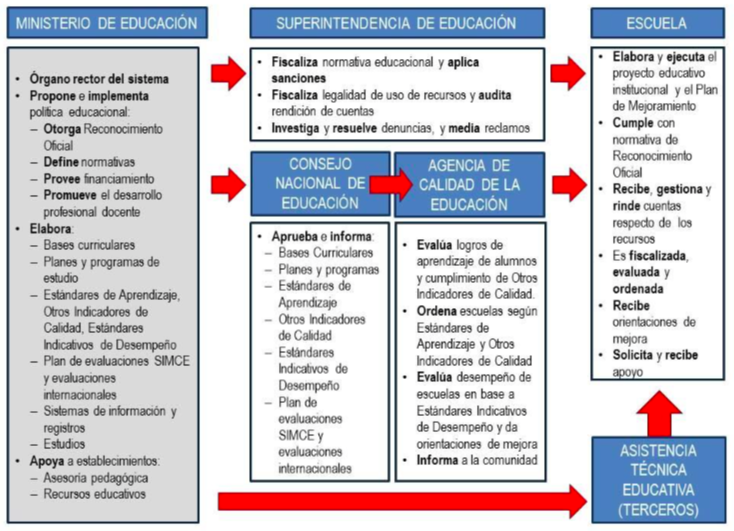
\includegraphics[width=0.8\textwidth]{Figuras/Institucionalidad}
      \caption{Esquema de la Institucionalidad del Sistema Educacional Chileno. Fuente: Centro de Estudios MINEDUC}
    \label{fig:esquema}
\end{figure}

Como es posible observar en la Figura~\ref{fig:esquema}, existe un trabajo en equipo entre las cuatro instituciones nombradas, donde la principal es el Ministerio de Educación de Chile, MINEDUC.

El MINEDUC es la entidad del Estado encargada de asegurar el acceso a la educación básica a toda la población; fomentar el desarrollo de la educación en todos sus niveles; estimular la investigación científica, tecnológica y la creación artística, y la protección e incremento del patrimonio cultural de la Nación. Es también la encargada de velar por los derechos de todos los estudiantes, pertenezcan estos a establecimientos públicos o privados. 


\textit{"La misión del Ministerio de Educación es asegurar un sistema educativo inclusivo y de calidad que contribuya a la formación integral y permanente de las personas y al desarrollo del país, mediante la formulación e implementación de políticas, normas y regulación, desde la educación parvularia hasta la educación superior."} \cite{misionmineduc}

Es función del Ministerio de Educación que el sistema integrado por los establecimientos educacionales financiado con recursos públicos provea una educación gratuita y de calidad, fundada en un proyecto educativo público laico, respetuoso y pluralista, que permita el acceso a toda la población y que promueva la inclusión social y la equidad. 

Específicamente, el Ministerio de Educación de Chile se organiza de la siguiente forma\cite{orgmineduc}:

\begin{description}
\item[Ministro de Educación] \hfill \\
El Ministro es el Jefe Superior del Ministerio y quien tiene directa relación con el Presidente de la República, junto a quien trabaja en las funciones de gobierno y administración del sector de educación y cultura.
Le corresponde dirigir las acciones educacionales y culturales concernientes al Estado.
\item[Subsecretaría de Educación] \hfill \\
La Subsecretaría es el órgano de colaboración directa del Ministro, cuya misión es administrar el Ministerio internamente y coordinar los órganos y servicios públicos del sector. También debe cumplir las funciones que en materias de su competencia le encomiende la ley y el Ministro. \\
El Subsecretario es el colaborador inmediato del Ministro, le corresponde coordinar y controlar las unidades que integran a la Subsecretaría. Actúa como ministro de fe del Ministerio y le corresponderán las atribuciones y obligaciones establecidas en la ley.
\item[Secretarías Regionales Ministeriales (SEREMI) de Educación] \hfill \\
Las Secretarías Regionales Ministeriales tienen como objetivo desconcentrar las funciones territorialmente. Cada una de las regiones administrativas de Chile cuenta con una Secretaría a cargo de un Secretario Regional Ministerial, quien es el representante del Ministerio en la región y actúa como colaborador directo del respectivo Intendente Regional.\\
La función de las SEREMIs es planificar, normar y supervisar el desarrollo del proceso educativo en los establecimientos ubicados en su territorio jurisdiccional, resguardando el cumplimiento de los objetivos y políticas educacionales y su correcta adecuación a las necesidades e intereses regionales. Les corresponderán, además, todas las funciones y atribuciones que las normas legales les otorgan, especialmente en materias técnico-pedagógicas y de inspección y control de subvenciones. 
\end{description}

\newpage

\begin{description}
\item[Centro de Estudios del MINEDUC] \hfill \\
Además, dentro del Ministerio de educación se encuentra el Centro de Estudios del MINEDUC, una institución que tiene como misión apoyar e informar, a través de la producción y difusión de conocimiento basado en evidencia, el proceso de toma de decisiones del Ministerio de Educación en materia de diseño, implementación y evaluación de políticas educativas. \cite{centroestudios}
\end{description}

Las tres entidades restantes que trabajan en conjunto con el Ministerio de Educación de Chile que se mencionan en la Figura~\ref{fig:esquema} se describen a continuación: 

\begin{description}
\item[Superintendencia de Educación] \hfill \\
La Superintendencia de Educación Escolar fue creada por la Ley número 20.529 sobre Sistema Nacional de Aseguramiento de la Calidad. Esta fue publicada el 27 de agosto de 2011 y entró en funcionamiento el 1 de septiembre de 2012. 
Su objetivo es fiscalizar, de conformidad a la ley, que los sostenedores de establecimientos educacionales reconocidos oficialmente por el Estado se ajusten a las leyes, reglamentos e instrucciones que dicte la Superintendencia, y fiscalizar la legalidad del uso de los recursos de los establecimientos que reciban aporte estatal. Además, debe proporcionar información, en el ámbito de su competencia, a las comunidades educativas y otros usuarios e interesados, y atender las denuncias y reclamos de éstos, aplicando las sanciones que en cada caso corresponda. \cite{superint}
\item[Consejo Nacional de Educación] \hfill \\
El Consejo Nacional de Educación es un organismo autónomo que, en lo referido a la educación escolar, se encarga de aprobar las bases curriculares, los planes y programas de estudio y el plan nacional de evaluaciones nacionales e internacionales de aprendizaje. También deberá aprobar los Estándares de Aprendizaje de los estudiantes, los Estándares Indicativos de Desempeño para los establecimientos educacionales y sus sostenedores, y la metodología de Ordenación de los establecimientos educacionales.
\item[Agencia de Calidad] \hfill \\
La Agencia de Calidad de la Educación, es una institución del Gobierno de Chile que tiene como objetivo  evaluar y orientar el sistema educativo para ayudar al mejoramiento de la calidad y equidad de las oportunidades educativas, es decir, que todo alumno tenga las mismas oportunidades de recibir una educación de calidad. Por ello, dos de sus funciones centrales son evaluar y orientar al sistema educativo para contribuir al mejoramiento de la calidad de las oportunidades educativas. \cite{agenciacalidad}
    \begin{description}
    \item [Sistema de Medición de la Calidad de la Educación] \hfill \\
    Tal como dice en sus objetivos, la Agencia de Calidad está encargada de evaluar al sistema de educación, y esto lo hace mediante el Sistema de Medición de la Calidad de la Educación, SIMCE, que es un conjunto de exámenes utilizados para medir el dominio de los estudiantes de temas del currículo escolar. Además recoge información sobre docentes, estudiantes, padres y apoderados a través de cuestionarios. Con esta información es posible contextualizar y analizar los resultados de los estudiantes en las pruebas SIMCE. 
    
    Las asignaturas que actualmente evalúa SIMCE son: Lenguaje y Comunicación ; Matemática; Ciencias Naturales; Historia, Geografía y Ciencias Sociales e Inglés. Estas pruebas son aplicadas a estudiantes de 2º, 4º, 6º y 8º básico, II  y III medio, y se informa oportunamente a los establecimientos las asignaturas que serán evaluadas en el año en curso, en el nivel que corresponda. Es importante mencionar que esta evaluación no se realiza de forma anual, por lo que existe una calendarización con los años en que se ha realizado y en qué niveles\footnote{La calendarización de las pruebas SIMCE se encuentra disponible en la web: http://www.agenciaeducacion.cl/simce/calendario-de-evaluaciones/}.
    
    Toda prueba SIMCE cuenta con tres tipos de encuestas, la primera es aquella que se aplica a los estudiantes para medir sus conocimientos en las diferentes asignaturas, otra es aplicada a los docentes de los alumnos que rinden la prueba, y una tercera se aplica a los apoderados de estos alumnos.
    \end{description}
\end{description}

\subsection{Otras Instituciones Relevantes}
Además de las instituciones nombradas recientemente, el Estado de Chile ha creado otras con la finalidad de trabajar junto al Ministerio y aportar con investigación, fiscalización, evaluación y todo lo que pueda beneficiar al sistema de educación del país y a sus actores. Los principales se enlistan a continuación, junto a una breve descripción de cada uno.

\begin{description}
\item[Junta Nacional de Auxilio Escolar y Becas (JUNAEB)] \hfill \\
La Junta Nacional de Auxilio Escolar y Becas es una institución pública del Estado de Chile cuya misión es velar por la igualdad de oportunidades ante la educación de niños y jóvenes que se encuentran en condiciones vulnerables económicamente. 
Se preocupa fundamentalmente de disponer de alimentación, becas, útiles escolares, entre otros, a todos los estudiantes que por desventajas económicas, sociales, psicológicas o biológicas lo necesitan. \cite{junaeb}
\item[Comisión Nacional de Investigación Científica y Tecnológica (CONICYT)] \hfill \\
CONICYT es una institución dependiente del Ministerio de Educación, fue creada en 1967 como organismo asesor de la Presidencia en materias de desarrollo científico. Sus grandes objetivos son dos: fomentar la formación de capital humano y el fortalecer la base científica y tecnológica del país. A su vez, ambos pilares son potenciados de manera transversal por un área de información científica y una de vinculación internacional. 
 Actualmente, el fomento a la formación de capital humano se traduce en el impulso de una política integral de formación, inserción y atracción de investigadores y profesionales de excelencia, así como de la promoción de una cultura científica en el conjunto de la sociedad, especialmente en el ámbito escolar. Por su parte, el fortalecimiento y desarrollo de la base científica y tecnológica implica una activa política de promoción de la investigación científica y el desarrollo tecnológico en todas las regiones del país, tanto a nivel individual como asociativo, y entre investigadores debutantes y consagrados, apoyo a centros de investigación de excelencia, promoción de alianzas entre investigación científica y sectores productivos, y fomento de investigación en áreas prioritarias y de interés público. \cite{conicyt}
\item[Junta Nacional de Jardines Infantiles (JUNJI)] \hfill \\
La Junta Nacional de Jardines Infantiles es una institución del Estado de Chile creada en 1970 por la Ley número 17.301, como un estamento autónomo vinculado al Ministerio de Educación y cuyo fin es atender la educación inicial del país.
Su objetivo es entregar Educación Parvularia de calidad a niños y niñas, preferentemente menores de cuatro años y en situación de vulnerabilidad social, para así generar las mejores condiciones educativas y contribuir a la igualdad de oportunidades. De este modo, esta institución ayuda al desarrollo de las capacidades, habilidades y aptitudes de los párvulos y apoya a las familias a través de los programas de atención educativa en salas cuna y jardines infantiles administrados en forma directa y por terceros.\cite{junji}
\item[Instituto Nacional de la Juventud (INJUV)] \hfill \\
El Instituto Nacional de la Juventud es un organismo de servicio público cuya misión consiste en colaborar con el Poder Ejecutivo en el diseño, planificación y coordinación de las políticas relativas a los asuntos juveniles.
Esta institución nació en el año 1991, y desde ese entonces se relaciona con el Presidente de la República a través del Ministerio de Desarrollo Social.
El trabajo del INJUV está orientado a jóvenes de entre 15 y 29 años, el cual consiste en coordinar políticas públicas de juventud que el Estado origina. A su vez, genera programas cuyos objetivos son fomentar la inclusión y participación social, el respeto de sus derechos y su capacidad de propuesta, poder de decisión y responsabilidad. \cite{injuv} 
\item[Dirección de Bibliotecas, Archivos y Museos (DIBAM)] \hfill \\
La Dirección de Bibliotecas, Archivos y Museos es un organismo público que se relaciona con el gobierno de Chile a través del ministerio de Educación, posee personalidad jurídica y patrimonio propio.
Fue creada el 18 de noviembre de 1929 por el Decreto con Fuerza de Ley número 5.200, y reúne a prestigiosas instituciones patrimoniales de todo el país. 
El Objetivo de esta institución es promover el conocimiento, la creación, la recreación y la apropiación permanente del patrimonio cultural y la memoria colectiva del país, para contribuir a la construcción de identidades y al desarrollo de las personas y de la comunidad nacional y de su inserción internacional. Lo anterior implica rescatar, conservar, investigar y difundir el patrimonio nacional, considerado en su más amplio sentido.\cite{dibam}
\end{description}

\subsection{Sistema Nacional de Evaluación del Desempeño de los Establecimientos Educacionales Subvencionados}

El Ministerio de Educación de Chile, en 1995 implementó el Sistema Nacional de Evaluación del Desempeño de los Establecimientos Educacionales Subvencionados, SNED, con el propósito de contribuir al mejoramiento de la calidad de la educación impartida por el sistema subvencionado del país.

En los años 2008-2009, los establecimientos técnico-profesionales regidos por el Decreto Ley Nº 3166 de 1980 fueron incorporados a la medición, y el beneficio se extendió a los profesores y asistentes de la educación de los establecimientos que resulten calificados como de excelente desempeño.

Esta herramienta busca ser un aporte a la trascendental tarea de mejorar la educación impartida en las aulas de clases chilenas, tomando en cuenta que una buena educación significa mayores oportunidades y progreso. Para cumplir con su objetivo, el SNED funciona mediante el incentivo y reconocimiento a los docentes y asistentes de la educación de los establecimientos con mejor desempeño en cada región. A través de este sistema se busca también que los padres y apoderados conozcan los resultados obtenidos y la evolución seguida por el establecimiento al que asisten sus hijos e hijas, y que los directivos, docentes y asistentes de la educación retroalimenten sus decisiones de gestión técnico-pedagógicas y administrativas.

El SNED contempla la entrega de un beneficio económico denominado Subvención por Desempeño de Excelencia, la cual se entrega en forma trimestral, a los sostenedores de los establecimientos educacionales seleccionados.

La normativa establece que los establecimientos beneficiarios deben representar a lo más el 35\% de la matrícula regional y que el monto que reciben debe destinarse integralmente a los profesionales de la educación que se desempeñan en dichos establecimientos. También que la selección de los establecimientos debe realizarse cada dos años y en la ley se fija un método para medir el desempeño.

Según la ley que crea el SNED, se debe considerar un conjunto de factores para la medición del desempeño de los establecimientos, que son los siguientes:

\begin{itemize}
    \item Efectividad, consiste en el resultado educativo obtenido por el establecimiento en relación con la población atendida.
    \item Superación, corresponde a los diferenciales de logro educativo obtenidos en el tiempo por el establecimiento educacional.
    \item Iniciativa, obedece a la capacidad del establecimiento para incorporar innovaciones educativas y comprometer el apoyo de agentes externos en su quehacer pedagógico.
    \item Mejoramiento de las condiciones de trabajo y adecuado funcionamiento del establecimiento.
    \item Igualdad de oportunidades, que corresponde a la accesibilidad y permanencia de la población escolar en el establecimiento educacional y la integración de grupos con dificultades de aprendizaje.
    \item Integración y participación de profesores y profesoras, padres y apoderados en el desarrollo del proyecto educativo del establecimiento.
\end{itemize}

Estos son los factores mediante los cuales se evalúa el desempeño de los establecimientos, principalmente respecto a los resultados alcanzados por sus alumnos y alumnas. Además existen otros aspectos del proceso educativo que se incorporan a esta evaluación, como la iniciativa, el mejoramiento en las condiciones de trabajo y del funcionamiento del establecimiento y la integración y participación de profesores y profesoras, padres y apoderados.

En el SNED se agrupa a los establecimientos de acuerdo a características externas que afectan los resultados obtenidos por ellos, de modo que su desempeño es comparado sólo al interior de cada grupo. Esta modalidad de agrupación, denominada grupos homogéneos, es un requisito técnico para la aplicación de la evaluación. Adicionalmente, para que los grupos homogéneos reflejen de mejor forma la realidad, su construcción se efectúa a nivel regional. Una vez determinados los grupos homogéneos, la evaluación se realiza de acuerdo a la medición de los indicadores seleccionados para cada uno de los factores, lo que se resume en la construcción de un valor numérico denominado Índice SNED.
A la fecha, se han efectuado nueve aplicaciones del SNED, desde el primer período bianual (1996- 1997) hasta el período 2012-2013. \cite{sned}

\subsection{Sistema Nacional de Aseguramiento de la Calidad de la Educación}
El Sistema Nacional de Aseguramiento de la Calidad de la Educación Escolar, SNAC, fue creado con la publicación de la Ley Nº 20529, promulgada el 11 de agosto de 2011. Establece el diseño de una nueva institucionalidad en educación, tal como se muestra anteriormente en la Figura~\ref{fig:esquema}. Esta comprende dos nuevos organismos: la Agencia de Calidad de la Educación y la Superintendencia de Educación.

La Agencia de Calidad tiene como fin evaluar los logros de aprendizaje, los Otros Indicadores de Calidad y el desempeño de las escuelas, para poder orientarlas en su quehacer institucional y pedagógico e informar a la comunidad escolar de estos procesos.

Esta ley también redefine algunas funciones del Ministerio de Educación, las que pasaron a ser desempeñadas íntegramente por la Agencia de Calidad y la Superintendencia de Educación Escolar. La Superintendencia tiene la tarea de fiscalizar el uso de los recursos y el cumplimiento de la normativa educacional, atender denuncias y reclamos, y establecer sanciones, de manera que las escuelas cumplan con las necesidades mínimas que los estudiantes requieren.

Este sistema busca asegurar el acceso a una educación de calidad con equidad para todos los estudiantes del país, mediante el apoyo y orientación constante a los establecimientos, así como la evaluación, y la fiscalización. \cite{sac}

\subsection{Ley de Subvención Escolar Preferencial}
En el año 2008 se establece la Ley de Subvención Escolar Preferencial, Ley SEP, cuya función es entregar recursos diferenciados por alumno vulnerable atendido e instituye un sistema más completo de responsabilización de resultados que el SNED, puesto que a los reconocimientos se le agregan sanciones. Los establecimientos, al suscribirse a la ley SEP, se comprometen a través de un Convenio de Igualdad de Oportunidades y Excelencia Educativa a cumplir ciertos requisitos, entre ellos: el cumplimiento de metas de efectividad del rendimiento académico acordadas con el Ministerio de Educación, la presentación y cumplimiento de un Plan de Mejoramiento Educativo, y el logro de los estándares nacionales para establecimientos. En este sistema los colegios son clasificados en tres categorías: autónomo, emergente y en recuperación, según el grado de consecución de los estándares nacionales definidos. Si un establecimiento se mantiene por más de cuatro años en recuperación el Ministerio de Educación le puede revocar el Reconocimiento Oficial, con lo queda inhabilitado para certificar estudios e imposibilitado para recibir subvención escolar.

Los factores definidos en la Ley SEP para clasificar a los establecimientos son:
\begin{itemize}
\item Resultados en las pruebas Simce en comparación a su grupo similar tomando en cuenta la distribución de resultados por Niveles de Logro.
\item Indicadores complementarios:
    \begin{itemize}
    \item Tasas de aprobación
    \item Tasas de retención
    \item Mejoramiento (como lo define el SNED)
    \item Integración de profesores, padres y apoderados (como lo define el SNED)
    \item Iniciativa (como lo define el SNED)
    \item En el caso de los establecimientos municipales, evaluación docente.
    \end{itemize}
\end{itemize}

Como es posible notar, ambos modelos de responsabilización implementados en Chile consideran el nivel socioeconómico al momento de evaluar y comparar el desempeño de los establecimientos. Además, se observa que ambos sistemas coinciden en la mayoría de los indicadores utilizados. La diferencia entre ambos sistemas radica en que el SNED busca reconocer el buen desempeño de los establecimientos y la clasificación SEP busca responsabilizar por resultados a todos los establecimientos y exigir rendición de cuentas de los recursos entregados.

\section{Identificación de necesidades y oportunidades}
En Chile está instaurado un sistema educativo que, tal como fue descrito anteriormente, permite la coexistencia de escuelas públicas y privadas. Refiriéndonos específicamente al sector público, resulta interesante lo que se obtiene al comparar este modelo educativo chileno con los requisitos de la educación pública que establece la UNESCO, ya que según esto la educación debe ser gratuita, de igual calidad para todos, promotora de la igualdad y no selectiva. Si bien en Chile se ha progresado en la medición de estándares mediante mapas de progreso, las pruebas SIMCE y otros, falta por avanzar en cuanto a lograr una educación más inclusiva y menos segregada socialmente. De hecho, en los últimos 20 años, más de 800 establecimientos educacionales municipales cerraron \cite{biobio} y según el INE, en el 2010 apenas el 32\% de los alumnos de la región metropolitana cursa su educación básica en colegios municipales \cite{ine}. 

Es por esto que el sistema educativo en Chile tiene ciertas falencias en el área pública. Es el MINEDUC el encargado de velar por que los establecimientos educacionales financiados con recursos públicos provean una educación gratuita y de calidad. Es por esto que, en este sentido, un punto muy importante es la finalización de la educación escolar, debido a las herramientas básicas que esta otorga. Resulta interesante cuantificar y encontrar patrones comunes de la deserción escolar. Para lograr esto se requiere identificar y entender los factores que desencadenan una salida del sistema escolar utilizando herramientas capaces de manejar mucha información y procesarla en tiempo real. Esto es posible, ya que existen diferentes fuentes de información pública disponible gracias a la Ley de Transparencia \cite{ley} actualmente vigente en Chile y tecnologías innovadoras para el manejo de grandes cantidades de datos.

Por lo tanto, en la educación pública de nuestro país, es posible identificar diferentes aristas que son importantes, como por ejemplo la brecha de la calidad de la educación entre escuelas públicas y privadas, la elección de la escuela a la que asistirán los alumnos, y la deserción escolar.

Siguiendo este camino, lo que se propone es la creación de una herramienta que tenga la capacidad de medir cuantitativamente la deserción escolar en el sector público\footnote{Sector público entendido como aquellos establecimientos que no son privados, es decir, en este caso se consideran solo aquellos establecimientos municipales y particulares subvencionados.} y señalar de forma temprana la deserción escolar a nivel institucional e individual en los establecimientos que pertenecen al sector recién mencionado.
Esta herramienta estará destinada a las autoridades que toman decisiones importantes para la educación del país a conocer y entender estos problemas para posteriormente poder enfrentarlos de la mejor forma posible, es decir, para el Ministerio de Educación de Chile y todas sus divisiones. 


\section{Objetivo general del proyecto y objetivos específicos}
El objetivo central es crear un prototipo de un sistema analítico en tiempo real, que entregue la información suficiente para identificar a los estudiantes con riesgo de desertar del sistema escolar o algún foco de deserción escolar. Esto ayudará a los encargados del diseño y desarrollo de políticas publicas para poder medir el impacto de estas sobre el sistema educativo.

A continuación se presentan los objetivos específicos del proyecto
\begin{itemize}
\item Identificar y comprender los diferentes factores que desencadenan salidas del sistema educativo (considerando aquellos establecimientos municipales y particulares subvencionados) para poder lograr un mejor desempeño de la herramienta
\item Crear modelos predictivos para poder detectar tempranamente el fracaso escolar
\item Implementar un prototipo funcional del sistema analítico en tiempo real
\end{itemize}

Para poder lograr los objetivos propuestos, se trabajará en conjunto al Centro de Investigación Avanzada en Educación (CIAE), cuya misión es realizar investigación científica de alto nivel que contribuya a mejorar la calidad y equidad de la educación en Chile \cite{ciae}.

Esta institución se encuentra actualmente trabajando para crear herramientas que apoyen el diseño, desarrollo y evaluación de las políticas en la materia de educación \cite{tools}. Específicamente, se  trabajará junto a sus investigadores, quienes son los encargados de canalizar la información disponible.

El CIAE, junto a un equipo multidisciplinario de la Universidad Adolfo Ibáñez se adjudicó el Segundo Concurso IDeA de Ciencia Aplicada FONDEF con el proyecto «\textit{Un prototipo de un sistema analítico e interactivo para apoyar el diseño, desarrollo y evaluación de políticas públicas en educación}» \cite{noticia}. 

Este proyecto abarca tres aristas importantes en la educación pública de Chile:
\begin{itemize}
    \item Deserción Escolar
    \item Desarrollo Territorial
    \item Selección de la Escuela a la cual se asistirá
\end{itemize}

Es precisamente aquí donde nace la iniciativa de la creación del sistema de alerta temprana para la deserción escolar, específicamente en el sector público. 

\section{Sumario}

En base a lo dicho en este primer capítulo, es posible formarse una idea de cuán compleja es la red de instituciones detrás de la educación chilena, lo que da cuenta de la importancia de generar un buen nivel de educación en el país. Es por eso que se hace necesario el apoyo mediante sistemas analíticos en tiempo real para que se puedan tomar buenas decisiones y crear políticas públicas en el área de educación que realmente respondan a los problemas actuales. 

Gracias a la ley de transparencia vigente en Chile es posible concretar estos objetivos, ya que se puede acceder a la información necesaria.

Lo que se verá en los capítulos siguientes es una extensa revisión bibliográfica con el fin de obtener una perspectiva completa sobre el saber acumulado respecto a la deserción escolar en establecimientos municipales de Chile. Posterior a esto se presenta la metodología que enmarcará el desarrollo del proyecto. Además, se realiza un análisis de las diferentes fuentes de información, los datos que se utilizarán y cómo estos se procesarán para luego proceder a la realización del modelo de predicción que permita llevar a cabo los objetivos propuestos. Finalmente, se dan a conocer los resultados obtenidos, las conclusiones y algunas recomendaciones para el sponsor y se concluye con el trabajo futuro.